\chapter{Feature Extraction}

%123456789 123456789 123456789 123456789 123456789 123456789 123456789 123456789

\label{ch:features}

In this chapter, we focus on the first step of the workflow described in the \autoref{sec:workflow}. The goal of this step is to represent useful information from an image of a tracked object in the form of a single feature vector. We aim to extract such feature vectors that would be close together (in terms of a suitable distance) if and only if they display the same person.

In this thesis, we use the feature vectors exclusively from the space of real numbers. Therefore, the form of the feature extraction function can be written as:

$$f : \mathcal{I} \goto \R^n \, \text{ for some } n \in \N$$

Where $\mathcal{I}$ is the space of images as in \autoref{eq:image}

\section{Histograms}

\label{sec:histograms}

The first set of feature extraction approaches focuses on encapsulating the distribution of color within a given image. The idea is that the color distribution of the tracked person's image should not change even if the given person moves within the display. We describe this distribution in the forms of histograms, similarly to other research (see \autoref{sec:early_research}).

% \begin{figure}
%     \centering
%     \def\svgwidth{\columnwidth}
%     \scalebox{0.6}{\input{img/histogram.pdf_tex}}
%     \caption[Visualization of histogram of data]{Visualization of histogram of data $(2, 3, 11, 15, 17, 23)$ with 3 bins, lower bound 0 and upper bound 30. The values of the histogram are $(2, 3, 1)$}
%     \label{fig:histogram}
%     \todo[inline=true]{Uhladit obrazek}
% \end{figure}

Histograms are often used for visualization purposes. However, in this work, we use histograms as actual feature vectors. To avoid any ambiguity, we offer the following definition, which is in line with the standard concept of histograms.% An example of histogram accompanied by standard visualization can be seen in \autoref{fig:histogram}.

\begin{defn}
\label{defn:simplehistogram}
Simple histogram of (multi)set $X \subset \R$ of n bins with lower bound $l$ and upper bound
$u$ is a vector $\vec{h}$ with following elements:
$$h_i = \abs{\left\{x \in X \mid l + (i-1) \cdot \frac{u-l}{n} \leq x < l + i \cdot \frac{u-l}{n}\right\}}$$
\end{defn}

However, defining histogram just over the multi-set of real numbers proves to be too restrictive for our needs. For example, in our standard representation of images, each pixel consists of three real numbers (color channels). Our original definition allows only to draw histograms out of a set of real numbers (rather than triplets of real numbers).

One way to circumvent this problem is to draw a histogram from each channel separately and concatenate them together. However, this naïve approach losses valuable information. For example, an image with half red and half green would generate the same histogram as an image that is half yellow (i.e., the combination of red and green) and half black (if we are using RGB channels).

Therefore, we shall use a bit more complex approach. An approach that would encapsulate the combined color information of each pixel. For this reason we use the following extension of simple histograms:

\begin{defn}
\label{defn:histogram}
Histogram of (multi)set $X \subset \R^m$ of n bins per channel with lower bound
$l$ and upper bound $u$ is a tensor $H$ with following elements:
$$H_{i_1, \ldots, i_m} = \abs{\left\{\vec{x} \in X \mid (\forall j) \left(l + (i_j-1) \cdot \frac{u-l}{n} \leq x_j < l + i_j \cdot \frac{u-l}{n}\right)\right\}}$$
\end{defn}

It is easy to see that the \autoref{defn:histogram} is (for $m = 1$)
consistent with the \autoref{defn:simplehistogram}.

Finally, as we may compare the histograms of images of various resolutions (and thus varying number of pixels), we shall use term of normalized histogram:

\begin{defn}
\label{defn:normhistogram}
Normalized, histogram of (multi)set $X \subset \R^m$ of n bins per channel with
lower bound $l$ and upper bound $u$ is a tensor $\widehat{H}$ with following
elements:
$$\widehat{H}_{i_1, \ldots i_m} = \frac{H_{i_1, \ldots i_m}}{\sum_{j_1, \ldots, j_m} H_{j_1, \ldots, j_m}}$$
Where $H_{i_1, \ldots, i_m}$ is a histogram of $X$.
\end{defn}

\subsection{Color Models}

As we mentioned previously in this section, so far, we aim to capture the distribution of the color within an image via histograms. However, we need to decide how we want to represent the pixels in the first place. We explore several well-known models.

\subsubsection{RGB}

The \autoref{defn:normhistogram} allows us to construct the first feature vector simply by following the definition. We can construct a (three-dimensional) histogram from the original channels (red, green, and blue).

However, such a naïve approach has significant drawbacks. In our scenario, it is common that the tracked object or person changes its brightness. It may move to a shadow or enter the area under a lamp. However, the object does not change its identity by moving to more bright areas. Therefore, we would prefer a model that is invariant to changes in the lightning (or at least not very sensitive). Unfortunately, this is not achieved by considering standard RGB as our color model.


A simple comparison can be seen in \autoref{fig:rubik_rgb_hsv}. In the figure, we work with three photos of the same object in three different light conditions. The original photos are shown in the top row. We can see the decomposition of red, green, and blue channels, respectively, in the following three rows. As we can see, even though we photographed the same object from the same vantage point, the changes in light conditions have a dramatic impact on all three channels.

\begin{figure}
    \newlength{\rubiklength}
    \newlength{\raiselength}
    \setlength{\rubiklength}{3cm}
    \setlength{\raiselength}{1.4cm}
    \centering
    \begin{tabular}{rccc}
         \raisebox{\raiselength}{Original} &
         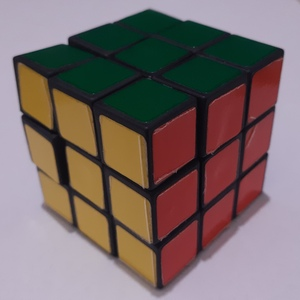
\includegraphics[width=\rubiklength]{img/rubik/1_orig.jpg} & 
         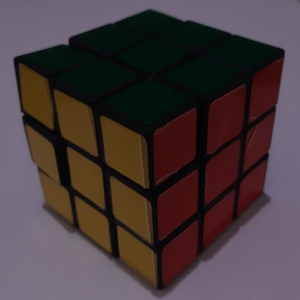
\includegraphics[width=\rubiklength]{img/rubik/2_orig.jpg} & 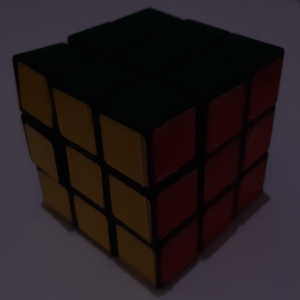
\includegraphics[width=\rubiklength]{img/rubik/3_orig.jpg}\\
         
         \raisebox{\raiselength}{Red} &
         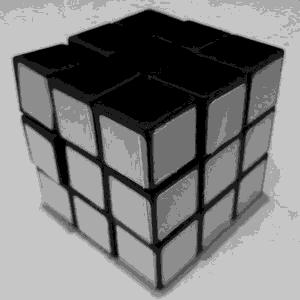
\includegraphics[width=\rubiklength]{img/rubik/1_rgb_r.jpg} & 
         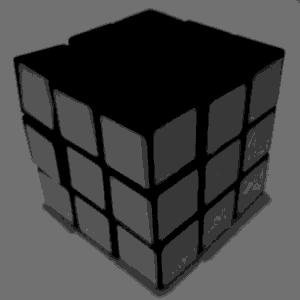
\includegraphics[width=\rubiklength]{img/rubik/2_rgb_r.jpg} & 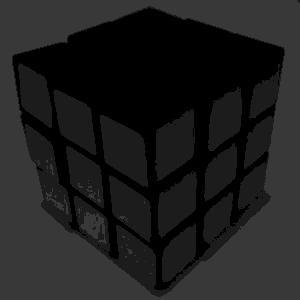
\includegraphics[width=\rubiklength]{img/rubik/3_rgb_r.jpg}\\
         
         \raisebox{\raiselength}{Green} &
         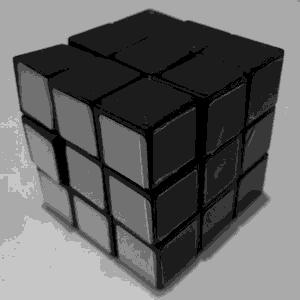
\includegraphics[width=\rubiklength]{img/rubik/1_rgb_g.jpg} & 
         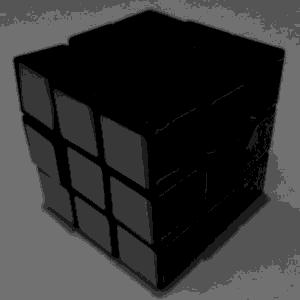
\includegraphics[width=\rubiklength]{img/rubik/2_rgb_g.jpg} & 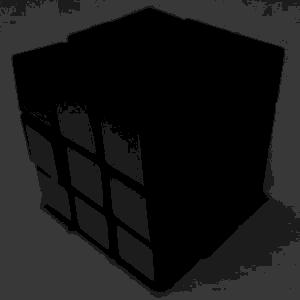
\includegraphics[width=\rubiklength]{img/rubik/3_rgb_g.jpg}\\
         
         \raisebox{\raiselength}{Blue} &
         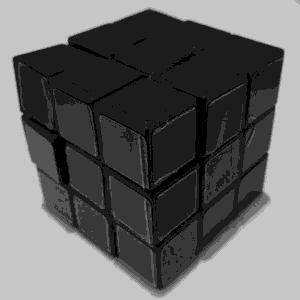
\includegraphics[width=\rubiklength]{img/rubik/1_rgb_b.jpg} & 
         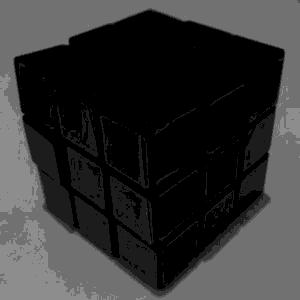
\includegraphics[width=\rubiklength]{img/rubik/2_rgb_b.jpg} & 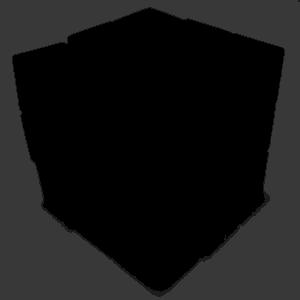
\includegraphics[width=\rubiklength]{img/rubik/3_rgb_b.jpg}\\
         
         \raisebox{\raiselength}{Hue} &
         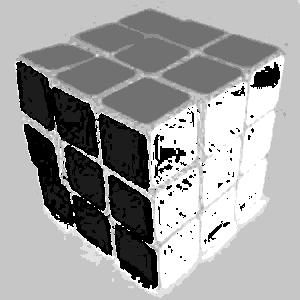
\includegraphics[width=\rubiklength]{img/rubik/1_hsv_h.jpg} & 
         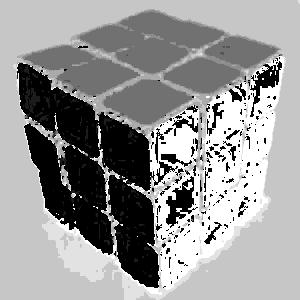
\includegraphics[width=\rubiklength]{img/rubik/2_hsv_h.jpg} & 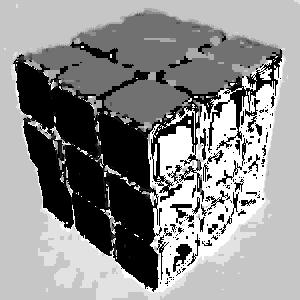
\includegraphics[width=\rubiklength]{img/rubik/3_hsv_h.jpg}\\
         
         \raisebox{\raiselength}{Saturation} &
         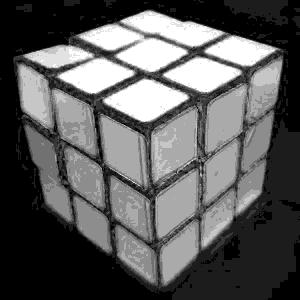
\includegraphics[width=\rubiklength]{img/rubik/1_hsv_s.jpg} & 
         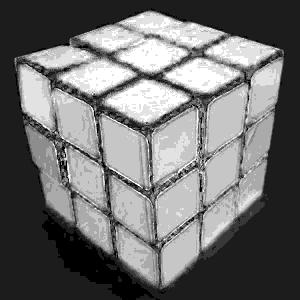
\includegraphics[width=\rubiklength]{img/rubik/2_hsv_s.jpg} & 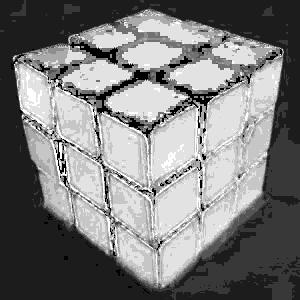
\includegraphics[width=\rubiklength]{img/rubik/3_hsv_s.jpg}\\
         
         \raisebox{\raiselength}{Value} &
         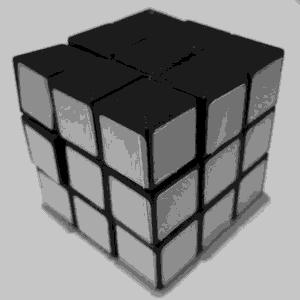
\includegraphics[width=\rubiklength]{img/rubik/1_hsv_v.jpg} & 
         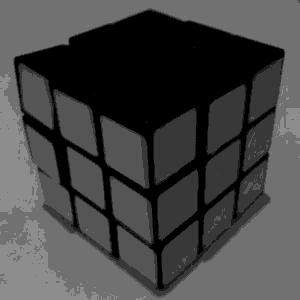
\includegraphics[width=\rubiklength]{img/rubik/2_hsv_v.jpg} & 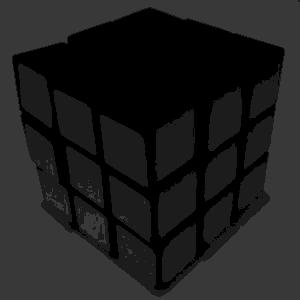
\includegraphics[width=\rubiklength]{img/rubik/3_hsv_v.jpg}

    \end{tabular}
    \caption[RGB and HSV decomposition of an object under varying light conditions]{RGB and HSV decomposition of an object under varying light conditions. The original photos are shown in the top row, the next three
    rows show red, green and blue components (lighter means higher value
    of given component). Last three rows show HSV components.}
    \label{fig:rubik_rgb_hsv}
\end{figure}

\begin{figure}
    \setlength{\rubiklength}{3cm}
    \setlength{\raiselength}{1.4cm}
    \centering
    \begin{tabular}{rccc}
         \raisebox{\raiselength}{Original} &
         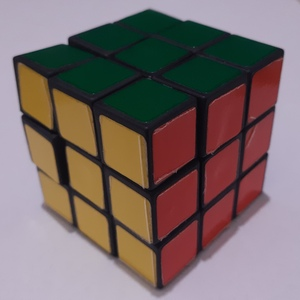
\includegraphics[width=\rubiklength]{img/rubik/1_orig.jpg} & 
         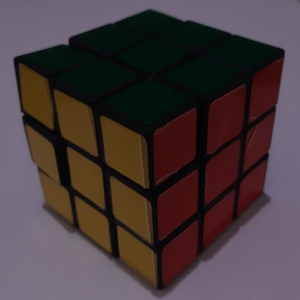
\includegraphics[width=\rubiklength]{img/rubik/2_orig.jpg} & 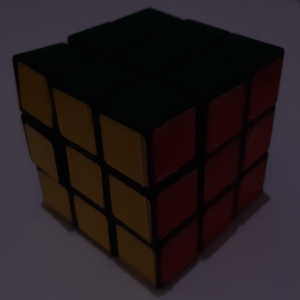
\includegraphics[width=\rubiklength]{img/rubik/3_orig.jpg}\\
         
         \raisebox{\raiselength}{Luma} &
         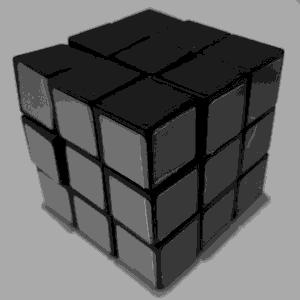
\includegraphics[width=\rubiklength]{img/rubik/1_yuv_y.jpg} & 
         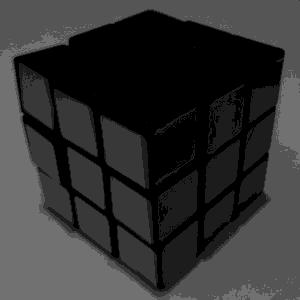
\includegraphics[width=\rubiklength]{img/rubik/2_yuv_y.jpg} &
         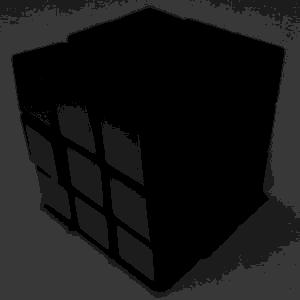
\includegraphics[width=\rubiklength]{img/rubik/3_yuv_y.jpg}\\
         
         \raisebox{\raiselength}{Blue projection} &
         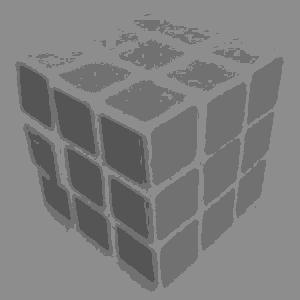
\includegraphics[width=\rubiklength]{img/rubik/1_yuv_u.jpg} & 
         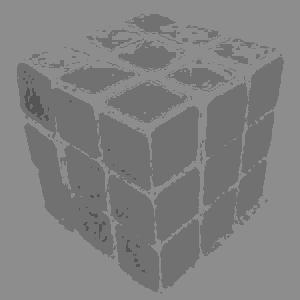
\includegraphics[width=\rubiklength]{img/rubik/2_yuv_u.jpg} &
         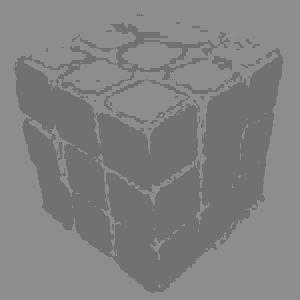
\includegraphics[width=\rubiklength]{img/rubik/3_yuv_u.jpg}\\
         
         \raisebox{\raiselength}{Red projection} &
         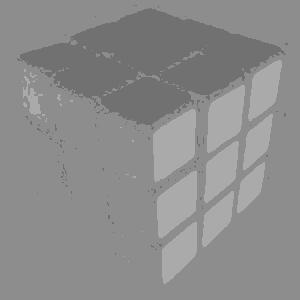
\includegraphics[width=\rubiklength]{img/rubik/1_yuv_v.jpg} & 
         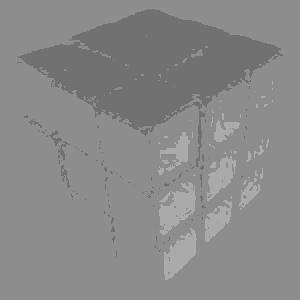
\includegraphics[width=\rubiklength]{img/rubik/2_yuv_v.jpg} & 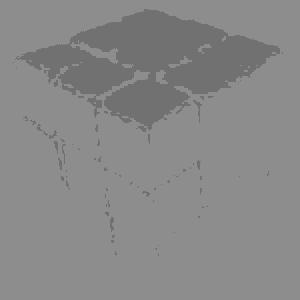
\includegraphics[width=\rubiklength]{img/rubik/3_yuv_v.jpg}
         \end{tabular}
    \caption[YUV decomposition of an object under varying light conditions]{YUV decomposition of an object under varying light conditions. The original photos are shown in the top row, remaining rows show components of luma (Y), blue projection (U) and red projection (V) respectively.}
    \label{fig:rubik_yuv}
\end{figure}

\subsubsection{HSV}

One of the possible remedies to tackle the problem of changes in the light conditions is to use another popular decomposition of color information -- hue, saturation, and value model. The last value is sometimes referred to as brightness resulting in the abbreviation HSB.\footnote{Another related decomposition is HSL, where the last channel is replaced by lightning. However, as the main channels for our purposes are the first two, we shall not discuss this differentiation any further.} General concept of HSV decomposition is displayed in \autoref{fig:hsv_cylinder}.

The first channel --- hue --- represents what we usually refer to as a main property of the color when we describe it. For example, colors with the hue of $60\degree$ we usually refer to as ``yellow'' and colors with the hue of $120\degree$ we refer to as ``green''.

The hue is often displayed as a direction or a position of the unit circle. Therefore, the unit of hue is most common a degree. This also means that the value of $359\degree$ and $0\degree$ represent nearly identical color (red).

Mathematically we can compute the value of hue from the RGB channels as
follows:

$$H = 60\degree \cdot x, \text{ where } x = 
\begin{cases}
0 & \text{ if } R = G = B \\
\frac{G - B}{R - B} & \text{ if } R \geq G \geq B \\
2 - \frac{R - B}{G - B} & \text{ if } G > R \geq B \\
2 + \frac{B - R}{G - R} & \text{ if } G \geq B > R \\
4 - \frac{G - R}{B - R} & \text{ if } B > G > R \\
4 + \frac{R - G}{B - G} & \text{ if } B > R \geq G \\
6 - \frac{B - G}{R - G} & \text{ if } R \geq B > G
\end{cases}$$

Another component of HSV is saturation. This component describes the ``colorfulness'' of the color. Colors with a low level of saturation always appear to be of grey shade, while the color with higher saturation changes depending on its hue component.

The value of saturation can be easily computed from the RGB components:

$$S = 1 - \frac{\max(R,G,B)}{\min(R,G,B)}$$

We can see that hue and saturation are quite robust in terms of changes in light conditions on the experiment in \autoref{fig:rubik_rgb_hsv}. Furthermore, they describe well the changes in the actual color of the material. That is at least for the simple example of the photo of a Rubik cube. The usefulness of these two channels in practical cases was shown by \cite{mckenna1997tracking}, where the authors used them to re-identify faces.

\begin{figure}
    \centering
    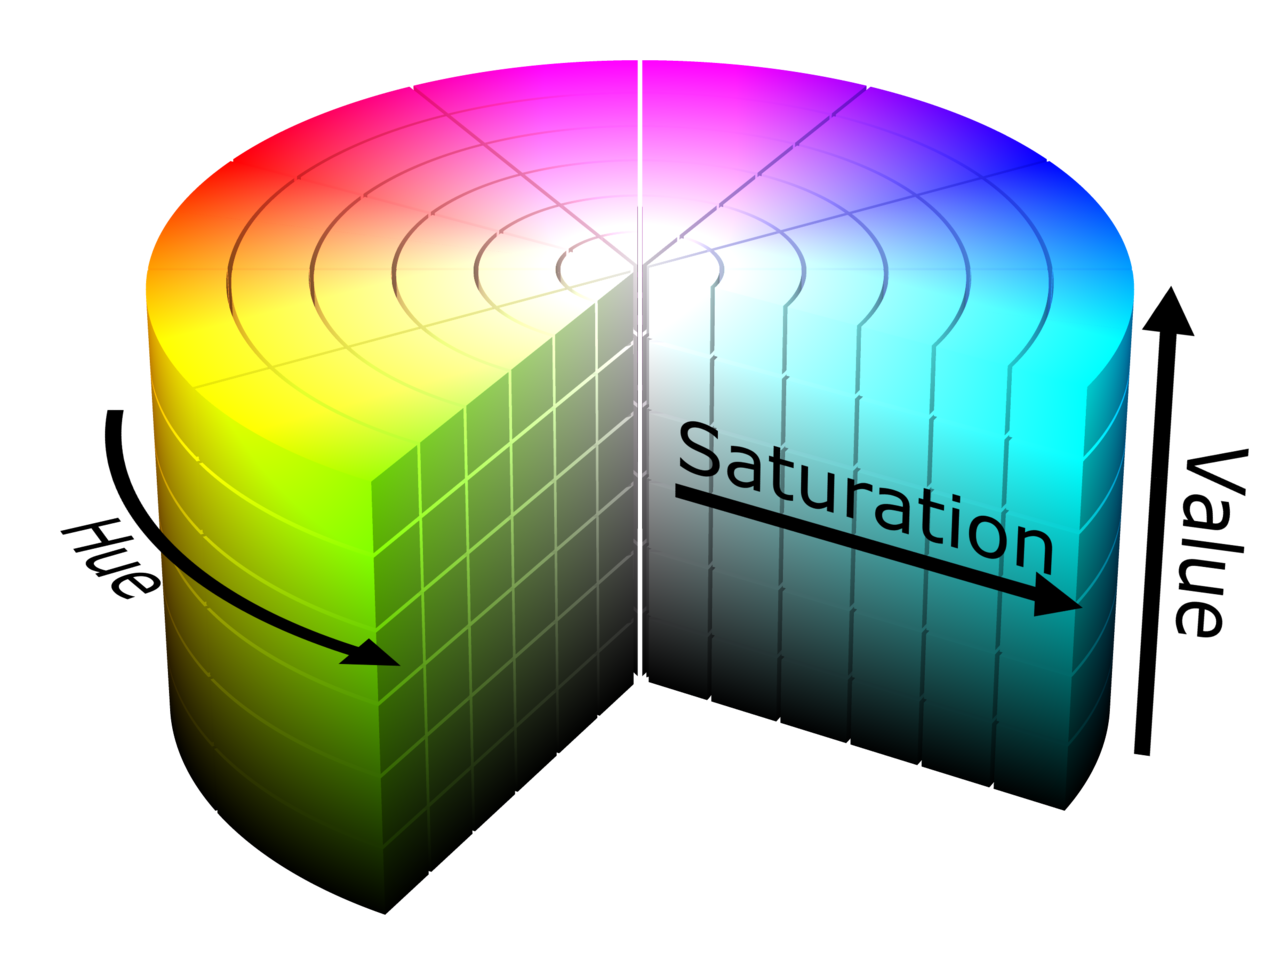
\includegraphics[width=6cm]{img/HSV_color_solid_cylinder.png}
    \caption[HSV color cylinder]{HSV color cylinder\\Source: HSV color solid cylinder\protect\footnotemark{} by SharkD, CC BY-SA 3.0\protect\footnotemark{}, via Wikimedia Commons}
    \label{fig:hsv_cylinder}
\end{figure}
\addtocounter{footnote}{-2}
\stepcounter{footnote}\footnotetext{\url{https://commons.wikimedia.org/wiki/File:HSV_color_solid_cylinder.png}}
\stepcounter{footnote}\footnotetext{\url{https://creativecommons.org/licenses/by-sa/3.0}}

\subsubsection{YUV}

Another fairly popular (\cite{orwell1999multi}, \cite{wren1997pfinder}) encoding of color used for this task is YCbCr (often referred as YUV) system. The first component, Y, represents the luminance (brightness) of the color\footnote{Component Y' is often used in place of the Y component. There is a difference between these two notation; however, we shall not discuss this difference further as the important components for our work is the latter two components.}. The remaining two components represent the chrominance of the color. The first of these two components (U or Cb) represents the blue projection. The last component (V or Cr) represents the red projection. The UV decomposition (with fixed Y) can be seen in \autoref{fig:yuv_decomposition}.

\begin{figure}
    \centering
    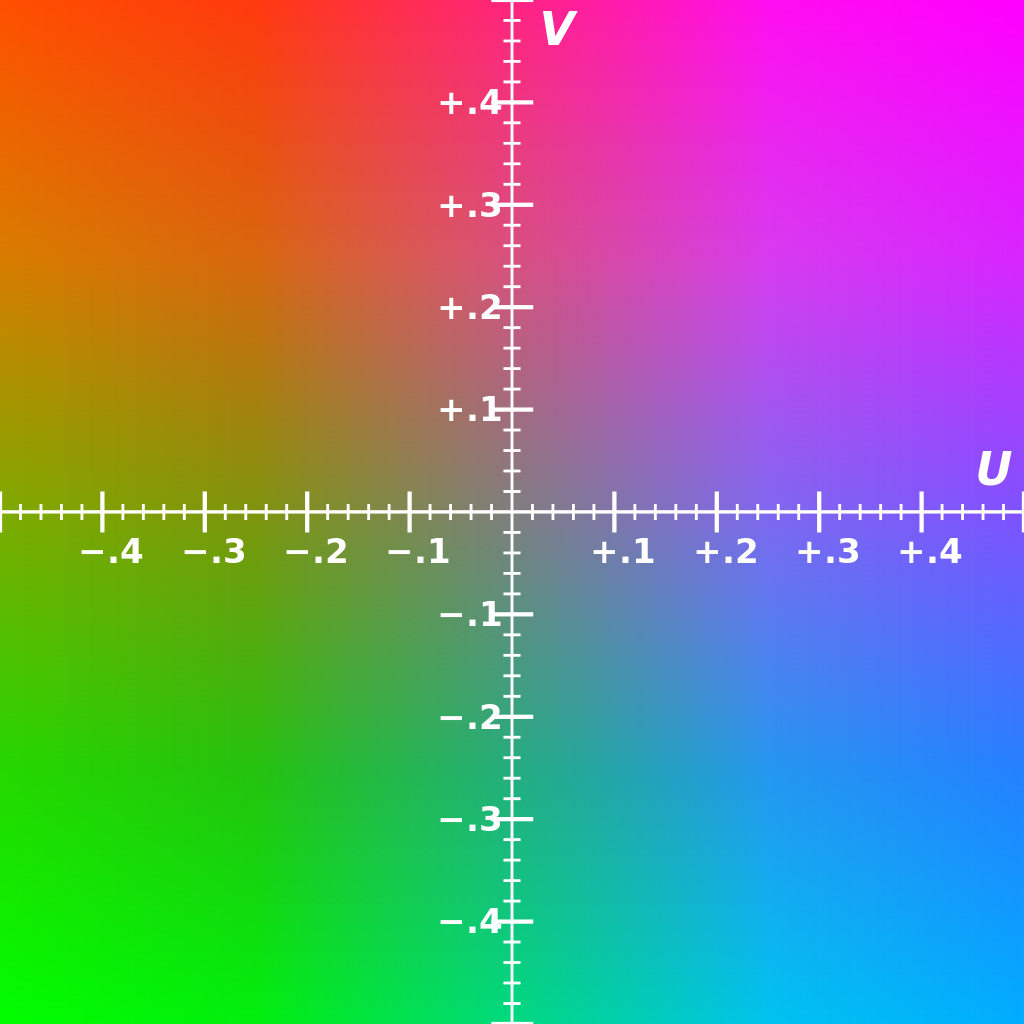
\includegraphics[width=5.6cm]{img/YUV_UV_plane.svg.png}
    \caption[UV plane of YUV decomposition]{UV plane of YUV decomposition\\
    Source: YUV UV plane\protect\footnotemark{} by Tonyle, CC BY-SA 3.0, via Wikimedia Commons \protect\footnotemark{}}
    \label{fig:yuv_decomposition}
\end{figure}
\addtocounter{footnote}{-2}
\stepcounter{footnote}\footnotetext{\url{https://commons.wikimedia.org/wiki/File:YUV_UV_plane.svg}}
\stepcounter{footnote}\footnotetext{\url{http://creativecommons.org/licenses/by-sa/3.0/}} 

The definition we use in this work comes from ITU-R Recommendation BT.601
(often just Rec. 601; \cite{bt2011studio}). However, we apply linear
transformation with offset and additional rounding to map the original space of U and V
to map these components to 8-bit values. This transformation can be expressed
as:

\begin{align*}
U &= \floor{(-43R - 84G + 127B) / 256} + 128 \\
V &= \floor{(127R - 106G - 21B) / 256} + 128
\end{align*}

How well these channels capture the color information and how much they change with the lightning change can be seen in the \autoref{fig:rubik_yuv}.

\subsection{Background Filtering}

There is another aspect to consider when using color histograms for generating feature vectors, and that is background filtering. If we did not filter out the background, the histogram might be polluted with useless information and may change during the tracked individual's movement, thus lowering the re-identification ability of the generated feature vector.

We evaluated the results without any background filtering at all as a baseline. Aside from that, we explore two rather simple approaches to this task. 

\subsubsection{Simple Crop}

The first, quite naïve approach is to crop from each image. We can remove strips of fixed width (relative to the image's dimension) from each side. An example of the result of this approach can be seen in \autoref{fig:crop_example}.

This way, we can remove (in most cases) all the background. Unfortunately, we often remove not only the background but also usually at least parts of the tracked individual. However, the basic idea is that the part of the person that remains after the crop should be mostly the same (i.e., displaying the same part) and not influenced by the background at all. Even though we may lose some information by this approach (i.e., if the crop from the bottom of the bounding box is too large, we may entirely crop-out the legs), we aim to verify if the remaining information is enough for re-identification purposes.

% \begin{figure}
%     \centering
%     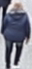
\includegraphics{img/background_filter/1_original.png}  \raisebox{0\height}{$\goto$} 
\includegraphics{img/background_filter/1_small.png} \hspace{2cm} 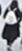
\includegraphics{img/background_filter/2_original.png} $\goto$ 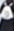
\includegraphics{img/background_filter/2_small.png}
%     \caption[An example of cropping on actual detections]{An example of cropping on actual detections. 20\% were cropped from left and right, 10\% from the top and 50\% from the bottom.}
%     \todo[inline=true]{\LaTeX{} zarovnat obrazky a sipky vertikalne}
%     \label{fig:crop_example}
% \end{figure}


\begin{figure}
    \centering
     \hfill
     \begin{subfigure}[t]{0.28\textwidth} % lady on the left
        \centering
        \begin{subfigure}[c]{0.3\textwidth}
          \centering
          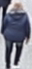
\includegraphics[]{img/background_filter/1_original.png}
        \end{subfigure}
        \hfill
        \begin{subfigure}[c]{0.3\textwidth}
          \centering
          $\goto$
        \end{subfigure}
        \hfill
        \begin{subfigure}[c]{0.3\textwidth}
          \centering
          
\includegraphics[]{img/background_filter/1_small.png}
        \end{subfigure}
     \end{subfigure}
     \hfill
     \begin{subfigure}[t]{0.28\textwidth} % lady on the right
        \centering
        \begin{subfigure}[c]{0.3\textwidth}
          \centering
          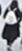
\includegraphics[]{img/background_filter/2_original.png}
        \end{subfigure}
        \hfill
        \begin{subfigure}[c]{0.3\textwidth}
          \centering
          $\goto$
        \end{subfigure}
        \hfill
        \begin{subfigure}[c]{0.3\textwidth}
          \centering
          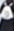
\includegraphics[]{img/background_filter/2_small.png}
        \end{subfigure}
     \end{subfigure}
     \hfill \hspace{0.1mm}

    \caption[An example of cropping on actual detections]{An example of cropping on actual detections. 20\% were cropped from left and right, 10\% from the top and 50\% from the bottom.}
    \label{fig:crop_example}
\end{figure}

\subsection{Weighting by Gaussian}

In the second approach, we assign each pixel a weight. This approach's idea is that the closer the pixel is to the center of the image, the more likely it is that the pixel represents part of the person rather than the background. Therefore, we want to assign higher importance to the pixels near the center.

There are many functions that would generate suitable weights (we need symmetric
function with single local maximum). However, we use one in particular
-- Gaussian (i.e. normal distribution function). We experiment with various
variations of the Gaussian as well as multiple vertical centering points.


To formalize the concept of weighted histograms we further alter the \autoref{defn:histogram}. In the original definition we simply counted the number of pixels corresponding to given bin (i.e. fulfilling the conditions). In the definition of weighted histogram instead of simply counting them, we sum the weights of corresponding histogram. Therefore, if we assign weight 1 to all pixels, resulting histogram would be the same as if we would not use weights at all:

\begin{defn}
\label{defn:weighted_histogram}
Weighted histogram of (multi)set $X \subset (\R^m \times \R)$ (where the last
element of the vector represents weight) of n bins per channel with
lower bound $l$ and upper bound $u$ is a tensor $H$ with following elements:
$$H_{i_1, \ldots, i_m} = \sum_{(\vec{x}, w) \in X} \left[w \text{ if } (\forall j) \left(l + (i_j-1) \cdot \frac{u-l}{n} \leq x_j < l + i_j \cdot \frac{u-l}{n}\right)\right]$$
\end{defn}

A visualization of this weighting can be seen in \autoref{fig:gaussian_weighting}.

\begin{figure}
    \centering
    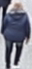
\includegraphics{img/background_filter/1_original.png} \hspace{1cm} 
\includegraphics{img/background_filter/weights.png} \hspace{1cm}
    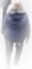
\includegraphics{img/background_filter/weights_applied.png}
    \caption[Visualization of background filtering by Gaussian weighting]{Visualization of background filtering by Gaussian weighting. The chosen distribution is horizontally centered and vertically offset to 30\% of height of the image. Chosen scale of the distribution is 0.3 (with respect to each respective dimensions of the image). The first image shows original image, the second weights, the last one represent applied weights (the weights are represent by transparency channel).}
    \label{fig:gaussian_weighting}
\end{figure}


\section{Neural Networks}



In this section, we explore feature vectors generated by neural networks. The information in these feature vector may not be as easy to understand as in case of using histograms. However, we aim to trade this lower level of explainability in hopes that the resulting feature vector would contain more useful information in terms of \reid{}.


\subsection{Custom Architecture}
\label{ssec:custom_architecture}

The first network we evaluate is a simple custom architecture. Our architecture is shallow compared to the more complex counter-parts that we also evaluate. It follows the usual practice of using alternating convolutional, max-pooling, and dropout layers with a dense layer prior to the output. For detailed description of the layers please consult \autoref{sec:conv} and \cite{deeplearningbook}. Detailed architecture is described in \autoref{tab:custom_architecture}.

\begin{table}
    \centering
    \begin{tabular}{l|l|l}
         Layer type & Parameters & Output shape \\ \hline
         \emph{Input} & & $n \times n \times 3$ \\
         Convolutional & filters: 64, kernel size: 2 & $n \times n \times 64$ \\
         Max-pooling & pool size: 2 & $\frac{n}{2} \times \frac{n}{2} \times 64$ \\
         Dropout & rate: 0.3 & $\frac{n}{2} \times \frac{n}{2} \times 64$ \\
         Convolutional & filters: 32, kernel size: 2 & $\frac{n}{2} \times \frac{n}{2} \times 32$ \\
         Max-pooling & pool size: 2 & $\frac{n}{4} \times \frac{n}{4} \times 32$ \\
         Dropout & rate: 0.3 & $\frac{n}{4} \times \frac{n}{4} \times 32$ \\
         Flatten & & 2$n^2$ \\
         Dense & output size: 256, without activation & 256 \\
         Normalization & & 256
    \end{tabular}
    \caption[Architecture of custom neural network]{Architecture of custom neural network. Parameter $n$ represents size of the input (the input is expected to be resized to $n\times n$ pixels, with RGB channels).}
    \label{tab:custom_architecture}
\end{table}

This simple architecture is not as complex as fine-tuned architectures such as ResNet and MobileNet. Therefore, we expect the resulting feature vectors to be a lower quality. However, it serves as a baseline for this type of approach. Furthermore, its simplicity has other advantages. Training takes significantly less time, which allows for a quick initial overview of the results. It also provides low latency during the inference, which is useful if we extend our usage to on-line \reid{}.

\subsection{Pre-trained Models}

\label{ssec:pretrained_models}

We experiment with various architectures based on the already trained \glspl{nn} (see \autoref{ssec:transfer_learning} and \autoref{sec:existing_architectures}).

The first experiment in this regard is to use ResNet and MobileNet as they were trained on the ImageNet dataset without the last ``classification'' layer. By such an experiment, we can hypothesize if these networks extract enough information simply by virtue of being image distinguishing neural networks or whether additional training is needed.

Finally, we explore the possibility of improving the abilities of \gls{nn} by fine-tuning them on our dataset. The first straight-forward approach we tested was to train the network without the last ``classification'' layer on our dataset without additional modification.\footnote{Actually, in order to employ Triplet Loss for learning, we needed to add a normalization layer. However, this layer does not add any trainable parameters.} However, we also explore the possibilities of slight modifications. We add a custom dense layer, sort of ``in place'' of the removed classification layer.

We also experiment with ``freezing'' the pre-trained part of the model. This means that we only fine-tuned the added final layer by learning, instead of the whole model. This has the advantage of a faster learning as the number of trainable parameters are significantly lower and the derivative has to be computed only for the last layer. Furthermore, using completely untrained weights in the final layer may cause the weights set in the pre-trained part to re-learn and completely lose the pre-trained model's advantages.

\subsection{Training}

We shall train and fine-tune presented models via gradient descent algorithm. To provide an unbiased estimation of the quality of the model in terms of \autoref{eq:mla}, we evaluate entirely different \gls{ses} than we used for training and fine-tuning. Both the training \gls{ses} and the \gls{ses} used for evaluation was created from our recordings. We have manually annotated extracted \glspl{det}. We describe the datasets more in \autoref{sec:datasets}.

For training itself, we use Triplet Loss as described in \autoref{sec:triplet_loss}. We extract the \gls{det} from single (``training'') \gls{ses} for the training purposes. As the goal of this step in the workflow is to obtain the representation of images, we discard all the metadata (e.g. position of the \gls{det}) and leave only the images of the \gls{det}.


Usually, we train the neural networks until the convergence of the loss function is reached. However, in some cases (notably, while incorporating the ResNet architecture), we needed to end the training earlier due to high hardware and time demands. Nevertheless, to avoid overfitting on the training dataset, we also evaluate the networks with weights learned in earlier training stages.

\subsection{Resizing Images}

\label{ssec:resizing}

Many \glspl{nn} for image processing (including those we work with) require the input image to be of fixed dimensions. For resizing images, various algorithms can be employed. We exclusively use the bicubic interpolation to achieve good results when scaling up (which is our common use case). For details please refer to \cite{keys1981cubic}. Other algorithms can be experimented with. However, it is out of the scope of this work.